\section{Descripción teórica} \label{sec:marco_teorico}

    Este trabajo se basa completamente en los libros de \cite{tomasi2003sistemas} y \cite{vela1999lineas}. 
    
    \subsection{Líneas de transmisión}

        Una línea de transmisión es un sistema de conductores metálicos para transferir energía eléctrica de un punto a otro. En forma más específica, una línea de transmisión consiste en dos o más conductores separados por un aislador, como por ejemplo un par de alambres o un sistema de pares de alambres. Una línea de transmisión puede tener desde unas pocas pulgadas hasta varios miles de millas de longitud. Se pueden usar las líneas de transmisión para propagar cd o ca de baja frecuencia, como la corriente eléctrica de 60 ciclos y las señales de audio; también se pueden usar para propagar frecuencias muy altas, como las señales de frecuencia intermedia y de radiofrecuencia. Cuando propagan señales de baja frecuencia, el comportamiento de una línea de transmisión es bastante sencillo y muy predecible; sin embargo, cuando propagan señales de alta frecuencia se complican las características de las líneas de transmisión, y su comportamiento es algo especial para un estudiante de circuitos y sistemas de elementos concentrados y constantes.

        \subsubsection{Ondas electromagnéticas transversales}

            La propagación de la energía eléctrica por una línea de transmisión se hace en forma de ondas electromagnéticas transversales (EMT). Una onda es un movimiento oscilatorio. La vibración de una partícula excita vibraciones semejantes en las partículas vecinas. Una onda EMT se propaga principalmente en el no conductor (dieléctrico) que separa los dos conductores de una línea de transmisión. En consecuencia, la onda viaja, o se propaga, a través de un medio. Para una onda transversal, la dirección del desplazamiento es perpendicular a la dirección de propagación. Una onda superficial de agua es una onda longitudinal. Una onda en la que el desplazamiento tiene la dirección de propagación se llama onda longitudinal. Las ondas sonoras son longitudinales. Una onda electromagnética (EM) se produce por la aceleración de una carga eléctrica. En un conductor, la corriente y el voltaje siempre se acompañan por un campo eléctrico E y un campo magnético H en la región vecina del espacio. La fig. \ref{fig:ondas_emt}-a muestra las relaciones espaciales entre los campos E y H de una onda electromagnética. En la fig. \ref{fig:ondas_emt}-b se ven los cortes transversales de los campos E y H que rodean a una línea de dos alambres paralelos.

        
            \begin{figure}[H]
                \centering
                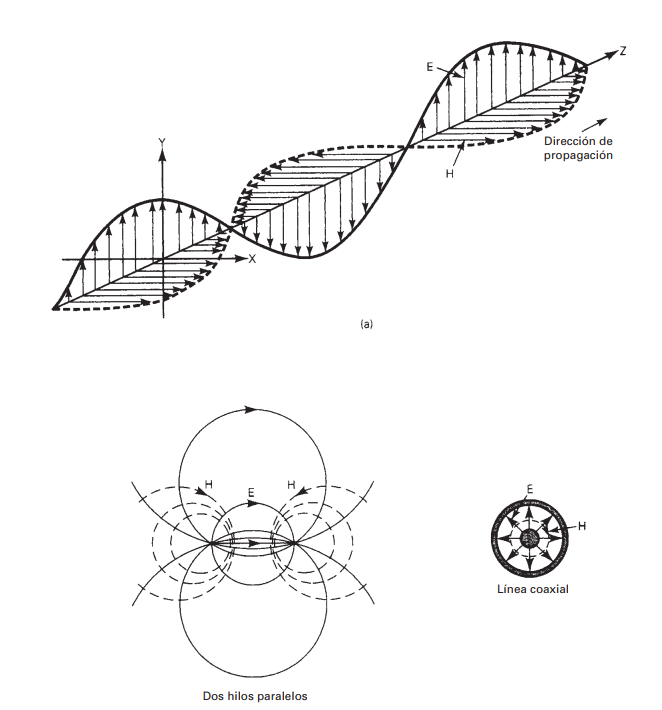
\includegraphics[width=0.8\textwidth]{imagenes/ondas_emt.png}
                \caption{Vistas: (a) en perspectiva; (b) transversal indicando el desplazamiento relativo de los campos E y H en una línea de transmisión}
                \label{fig:ondas_emt}
            \end{figure}

        \subsubsection{Tipos de líneas de transmisión}

            En general, las líneas de transmisión se pueden clasificar en:

            \begin{itemize}
                \item \textbf{Balanceadas}
                \item \textbf{Desbalanceadas}
            \end{itemize}

            \paragraph{1. Balanceadas:}

            En las líneas balanceadas de dos alambres ambos conductores llevan corriente; uno lleva la señal y el otro es el regreso. Este tipo de transmisión se llama transmisión diferencial o balanceada de señal. La señal que se propaga por el alambre se mide como diferencia de potencial entre los dos conductores.

            \begin{figure}[H]
                \centering
                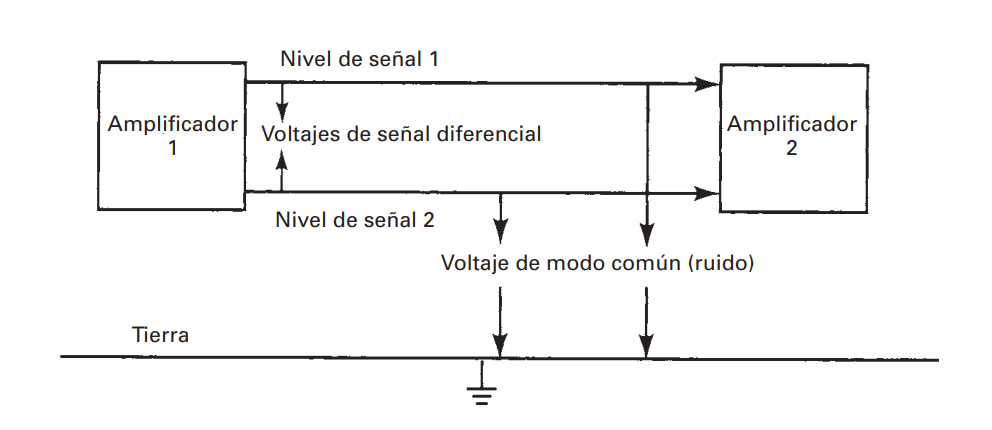
\includegraphics[width=0.8\textwidth]{imagenes/balanceadas.png}
                \caption{Sistema de transmisión diferencial o balanceado}
                \label{fig:balanceadas}
            \end{figure}

            La fig. \ref{fig:balanceadas} muestra un sistema de transmisión balanceado. Ambos conductores de una línea balanceada conducen corriente de señal, y las corrientes tienen igual magnitud con respecto a la masa o tierra eléctrica, pero viajan en direcciones opuestas. Las corrientes que fluyen en direcciones opuestas en un par balanceado de alambres se llaman corrientes de circuito metálico. Las corrientes que tienen las mismas direcciones se llaman corrientes longitudinales. Un par balanceado de alambres tiene la ventaja de que la mayor parte del ruido de interferencia (que a veces se llama voltaje de modo común) se induce por igual en ambos conductores, y produce corrientes longitudinales que se anulan en la carga. La anulación de las señales de modo común se llama rechazo de modo común (CMR, de common-mode rejection). Son comunes las relaciones de rechazo de modo común (CMRR, de common-mode rejection ratio) de 40 a 70 dB.

            Todo par de alambres puede trabajar en el modo balanceado, siempre que ninguno de ellos esté al potencial de tierra. Aquí se incluye el cable coaxial que tiene dos conductores centrales y un blindaje. En general, el blindaje se conecta a tierra para evitar que la interferencia estática penetre a los conductores centrales.

            \begin{figure}[H]
                \centering
                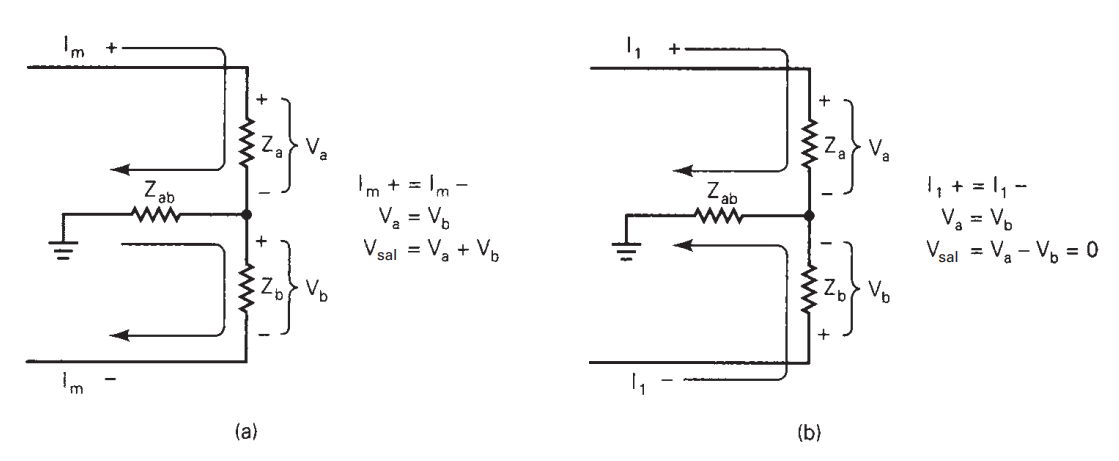
\includegraphics[width=0.8\textwidth]{imagenes/corriente_cmrr.png}
                \caption{Resultados de corrientes metálicas y longitudinales en una línea de transmisión balanceada: (a) corrientes metálicas debidas a voltajes de señal; (b) corrientes longitudinales debidas a voltajes de ruido}
                \label{fig:corriente_cmrr}
            \end{figure}

            La fig. \ref{fig:corriente_cmrr} muestra el resultado de las corrientes metálicas y longitudinales en una línea de transmisión. Se ve que las corrientes longitudinales, que se producen con frecuencia debido a la interferencia de estática, se anulan en la carga.

            \paragraph{2. Desbalanceadas:}

            En una línea de transmisión desbalanceada, un alambre está al potencial de tierra, mientras que el otro tiene el potencial de una señal. A este tipo de transmisión se le llama transmisión de señal desbalanceada o asimétrica. En la transmisión desbalanceada, el alambre de tierra puede ser también la referencia para otros conductores portadores de señal. Si ése es el caso, el alambre de tierra debe ir donde vaya cualquiera de los conductores de señal. A veces esto origina problemas, porque un tramo de alambre tiene resistencia, inductancia y capacitancia y, en consecuencia, puede existir una pequeña diferencia de potencial entre dos puntos cualesquiera en el conductor de tierra. En consecuencia, ese conductor no es un punto de referencia perfecto, y puede tener ruido inducido en él. Un cable coaxial normal de dos conductores es una línea desbalanceada. El segundo conductor es el blindaje, que casi siempre se conecta a tierra.

            \begin{figure}[H]
                \centering
                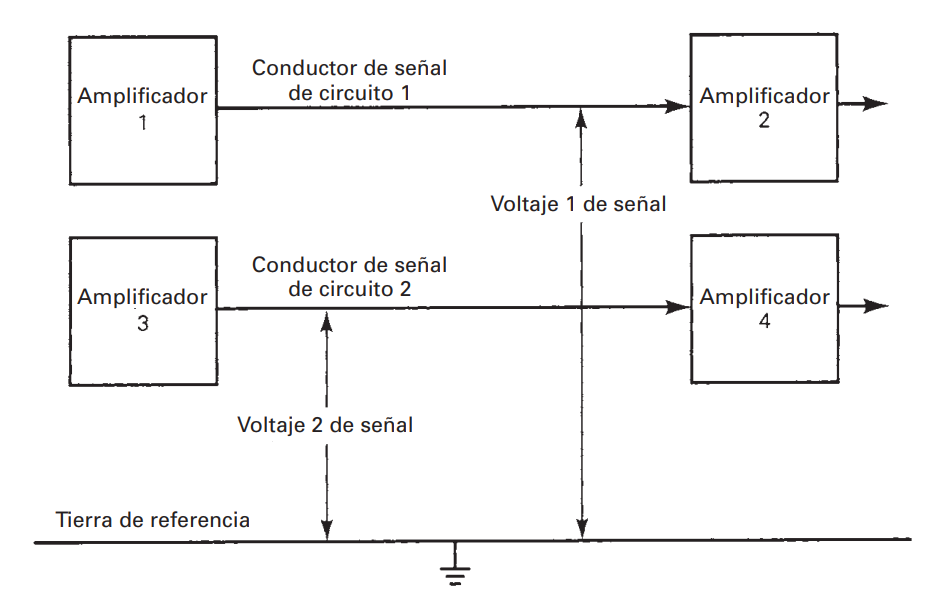
\includegraphics[width=0.8\textwidth]{imagenes/desbalanceado.png}
                \caption{Sistema de transmisión asimétrico o desbalanceado}
                \label{fig:desbalanceado}
            \end{figure}

            La fig. \ref{fig:desbalanceado} muestra dos sistemas desbalanceados de transmisión. La diferencia de potencial en cada alambre de señal se mide entre él y la tierra. Las líneas de transmisión balanceadas se pueden conectar a líneas desbalanceadas, y viceversa, con transformadores especiales llamados balunes.

        \subsubsection{Balunes}

            Un dispositivo que se usa para conectar una línea de transmisión balanceada con una carga desbalanceada se llama balún (balanceado a desbalanceado, de balanced to unbalanced). También, lo que es más común, una línea de transmisión desbalanceada, como un cable coaxial, se puede conectar con una carga balanceada, como una antena, mediante un transformador especial con desbalanceado primario y devanado secundario con toma central. El conductor externo (blindaje) de una línea de transmisión desbalanceada se suele conectar a tierra. A frecuencias relativamente bajas se puede usar un transformador ordinario para aislar la tierra de la carga, como se ve en la fig. \ref{fig:balunes}-a. El balún debe tener un blindaje electrostático conectado a tierra física, para reducir al mínimo los efectos de las capacitancias parásitas.

            \begin{figure}[H]
                \centering
                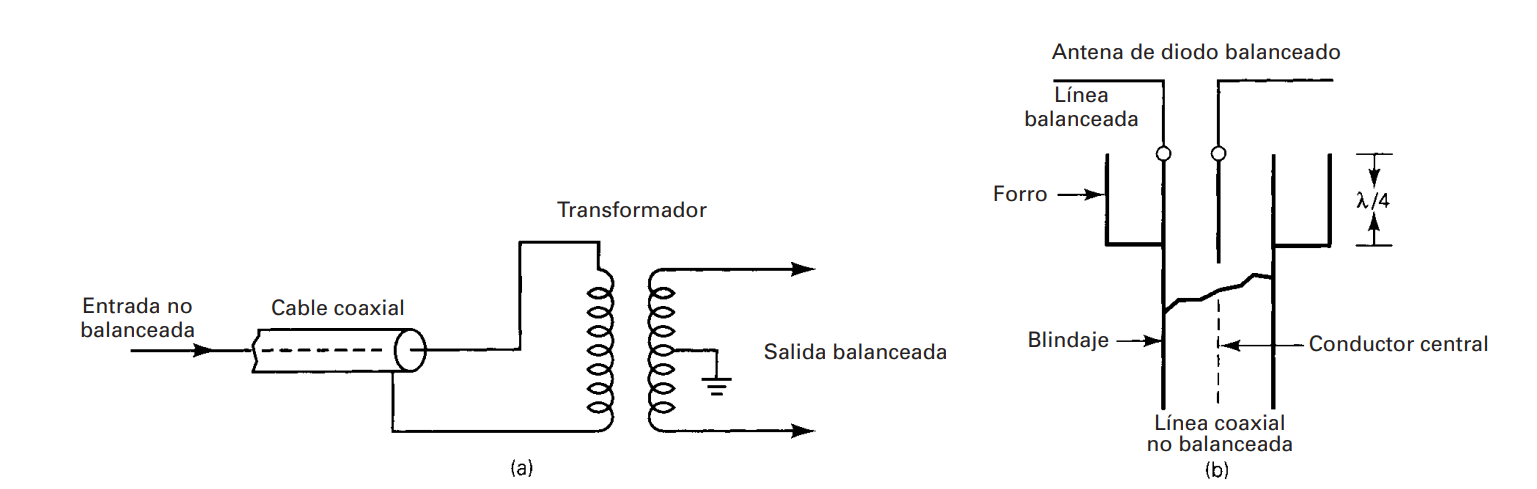
\includegraphics[width=\textwidth]{imagenes/balunes.png}
                \caption{Balunes: (a) balún de transformador; (b) balún de bazuca}
                \label{fig:balunes}
            \end{figure}

            Cuando las frecuencias son relativamente altas se usan balunes de varios tipos para líneas de transmisión. El más común es el balún de banda angosta, que a veces se llama choke, forro o balún bazuca, y se ve en la fig. 8-6b. Un choke de cuarto de onda se instala en torno al conductor externo de un cable coaxial y se conecta con él. Así, la impedancia que se ve hacia la línea de transmisión se forma por el choke y el conductor externo, y es igual a infinito, es decir, el conductor externo ya no tiene impedancia cero a tierra. Por lo anterior, un alambre del par balanceado se puede conectar con el choke sin poner en corto la señal. El segundo conductor se conecta al conductor interno del cable coaxial.

        \subsubsection{Líneas de transmisión de conductores paralelos}

            \begin{figure}[H]
                \centering
                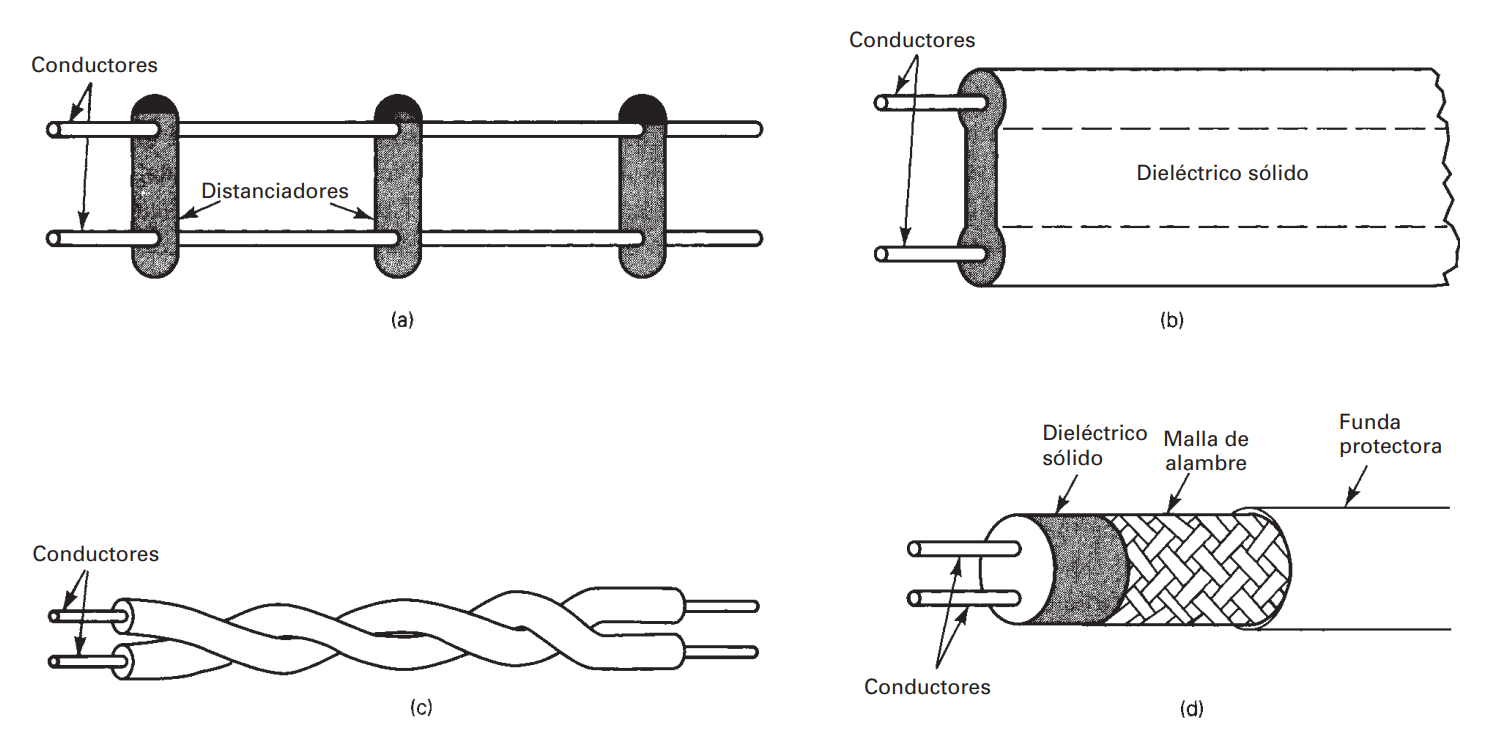
\includegraphics[width=0.8\linewidth]{imagenes/tipos_lineas.png}
                \caption{Líneas de transmisión: (a) alambres desnudos; (b) conductores gemelos; (c) par trenzado; (d) par blindado}
                \label{fig:tipos_lineas}
            \end{figure}

            \paragraph{a. Línea de transmisión de alambre desnudo:}

            Una línea de transmisión de alambre desnudo es un conductor de dos alambres paralelos; se ve en la fig. \ref{fig:tipos_lineas}-a. Consiste simplemente en dos alambres paralelos a corta distancia y separados por aire. Se colocan espaciadores no conductores a intervalos periódicos, para sostenerlos y mantener constante la distancia entre ellos.
            La distancia entre los dos conductores en general es entre 2 y 6 pulgadas. El dieléctrico no es más que el aire entre y en torno a los dos conductores en los que se propaga la EMT. La única ventaja real de este tipo de línea de transmisión es su construcción sencilla. Como no tiene blindaje, las pérdidas por radiación son altas y es susceptible de captar ruido. Son las principales desventajas de una línea de transmisión de cable desnudo. Por consiguiente, estas líneas se trabajan normalmente en el modo balanceado.

            \paragraph{b. Conductores gemelos:}

            Los conductores gemelos son otra forma de línea de transmisión de dos alambres paralelos, y se ve en la fig. \ref{fig:tipos_lineas}-b. A los conductores gemelos también se les llama con frecuencia cable de cinta. Los conductores gemelos son, en esencia, lo mismo que la línea de transmisión de conductores desnudos, pero los distanciadores entre los dos conductores se reemplazan con un dieléctrico macizo continuo. Así se asegura la distancia uniforme a lo largo de todo el cable, lo cual es una buena característica. En forma normal, la distancia entre los dos conductores es 5/16 de pulgada para el cable de transmisión de TV. Los materiales dieléctricos más frecuentes son el teflón y el polietileno.

            \paragraph{c. Cable de par trenzado:}

            Un cable de par trenzado se forma torciendo entre sí dos conductores aislados. Con frecuencia, los pares se trenzan en unidades y las unidades se llevan en núcleos que a su vez se cubren con varios tipos de forros, dependiendo de la aplicación. Los pares vecinos se trenzan con distintos pasos (longitud de torcimiento) para reducir la interferencia debida a la inducción mutua entre los pares. Las constantes primarias del cable de par trenzado son sus parámetros eléctricos: resistencia, inductancia, capacitancia y conductancia, que están sujetas a variaciones de acuerdo con el ambiente físico, como temperatura, humedad y esfuerzos mecánicos, y dependen de las diferencias de manufactura. En la fig. \ref{fig:tipos_lineas}-c se muestra un cable de par trenzado.

            \paragraph{d. Par de cable blindado:}

            Para reducir las pérdidas por radiación y la interferencia, con frecuencia las líneas de transmisión se encierran en una malla de alambre metálica y conductora. La malla se conecta a tierra y funciona como blindaje. También, la malla evita que se irradien señales fuera de ella, y evita que la interferencia electromagnética llegue a los conductores de señal. En la fig. \ref{fig:tipos_lineas}-d se ve un par de cable blindado. Está formado por dos alambres conductores paralelos separados por un material dieléctrico macizo. Toda la estructura se encierra en un tubo de conductor integrado por una malla, y después se cubre con una capa protectora de plástico.


        \subsubsection{Líneas de transmisión concéntricas o coaxiales}

            \begin{figure}[H]
                \centering
                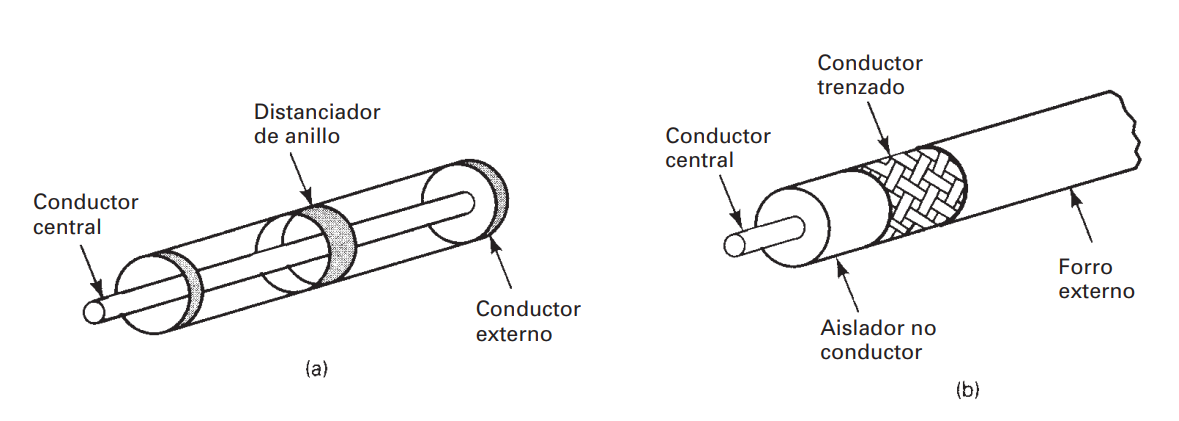
\includegraphics[width=0.8\textwidth]{imagenes/coaxiales.png}
                \caption{Líneas de transmisión concéntricas o coaxiales: (a) rígida llena de aire; (b) línea maciza flexible}
                \label{fig:coaxiales}
            \end{figure}

            Las líneas de transmisión de conductores paralelos son adecuadas para aplicaciones en baja frecuencia. Sin embargo, con las\textbf{ altas frecuencias aumentan demasiado sus pérdidas por radiación y en dieléctrico, así como su susceptibilidad a la interferencia externa}. Por lo anterior, \textbf{se usan mucho los conductores coaxiales} en aplicaciones de alta frecuencia, \textbf{para reducir las pérdidas y para aislar las trayectorias de transmisión}. El cable coaxial básico consiste en un conductor central rodeado por un conductor externo concéntrico, a distancia uniforme del centro. A frecuencias de trabajo relativamente altas, el conductor externo coaxial proporciona un excelente blindaje contra la interferencia externa. Sin embargo, no es económico usar un blindaje con frecuencias relativamente bajas. También, casi siempre el conductor externo de un cable coaxial se conecta a tierra, y eso limita su empleo a aplicaciones desbalanceadas o asimétricas.

            En esencia hay dos tipos de cables coaxiales: líneas rígidas llenas de aire o líneas flexibles macizas. La fig. \ref{fig:coaxiales}-a muestra una línea coaxial rígida de aire. Se ve que el conductor central está coaxialmente rodeado por un conductor externo tubular, y que el material aislador es aire. El conductor externo está aislado físicamente, y separado del conductor central por un distanciador, que puede ser de vidrio pyrex, poliestireno o algún otro material no conductor. La fig. \ref{fig:coaxiales}-b representa un cable coaxial flexible y macizo. El conductor externo es una malla de alambre flexible, y es coaxial respecto al conductor central. El material aislante es polietileno macizo no conductor, que proporciona tanto soporte como aislamiento eléctrico entre los conductores interno y externo. El conductor interno es un alambre flexible de cobre, que puede ser macizo o hueco.

            Es relativamente costoso fabricar los cables coaxiales rígidos de aire, y para minimizar las pérdidas, el aislador de aire debe estar relativamente libre de humedad. Los cables coaxiales macizos tienen menos pérdidas y son más fáciles de fabricar, instalar y mantener. Los dos tipos de cable coaxial son relativamente inmunes a la radiación externa, irradian poco ellos mismos, y pueden funcionar a mayores frecuencias que sus contra partes de conductores paralelos. Las desventajas básicas de las líneas coaxiales de transmisión son su alto costo y que se deben usar en el modo desbalanceado.

        \subsubsection{Tabla de AWG}

            El sistema AWG en cables eléctricos, significa American Wire Gauge, traduciendo al español es el Calibre de Alambre Estadounidense. Los cables de estándar AWG son para uso residencial y su aplicación data desde 1857, en particular es para conductores redondos, sólidos no ferrosos.
            
            En el sistema AWG mientras mayor sea el número, más delgado es el hilo del diámetro, ya que el calibre nos indica el número de veces que el metal necesita ser sometido a las hileras de trefilado para llegar al diámetro deseado. Y los números más bajos son para indicar cables más gruesos. Por ejemplo, el cable 4 AWG es más grueso que el cable 18 AWG. Son 44 los tamaños que se encuentran estandarizados en sistema AWG.

            \begin{figure}[H]
                \centering
                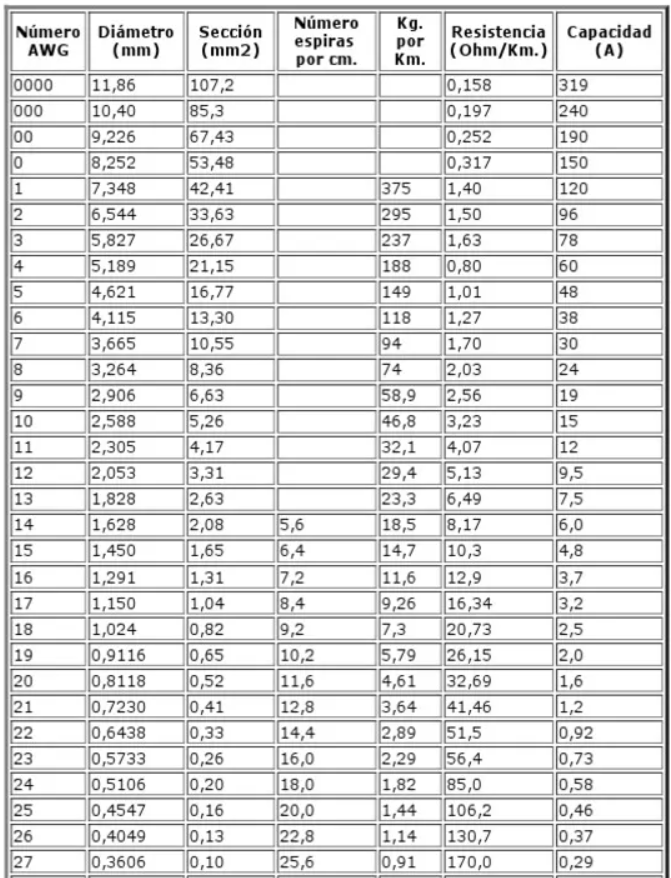
\includegraphics[width=0.5\linewidth]{imagenes/awg.png}
                \caption{Valores normalizados de cables AWG}
                \label{fig:awg}
            \end{figure}

        \subsubsection{Circuito equivalente de una línea de transmisión}

            \paragraph{Líneas uniformemente distribuidas:}

            Las características de una línea de transmisión están determinadas por sus propiedades eléctricas, como por ejemplo la conductividad de los alambres y la constante dieléctrica del aislamiento, y de sus propiedades físicas, como diámetro del alambre y distancia entre conductores. Estas propiedades, a su vez, determinan las constantes eléctricas primarias: resistencia de cd en serie \textbf{(R)}, inductancia en serie \textbf{(L)}, capacitancia en paralelo \textbf{(C)} y conductancia en paralelo \textbf{(G)}. A lo largo de la línea hay resistencia e inductancia, mientras que entre los dos conductores se desarrollan capacitancia y conductancia. Las constantes primarias se distribuyen uniformemente en toda la longitud de la línea y, en consecuencia, se les llama parámetros distribuidos. Para simplificar el análisis, los parámetros distribuidos se agrupan entre sí por unidad de longitud, para formar un modelo eléctrico artificial de la línea. Por ejemplo, la resistencia en serie se especifica en general en ohms por unidad de longitud (por ejemplo, ohms por metro).

            La fig. \ref{fig:circ_lt} muestra el circuito eléctrico equivalente de una línea de transmisión metálica de dos conductores, donde se muestra la colocación relativa de los diversos parámetros agrupados. La conductancia entre los dos alambres se muestra en su forma recíproca, y se menciona como resistencia de fugas en paralelo, $R_s$.

            \begin{figure}[H]
                \centering
                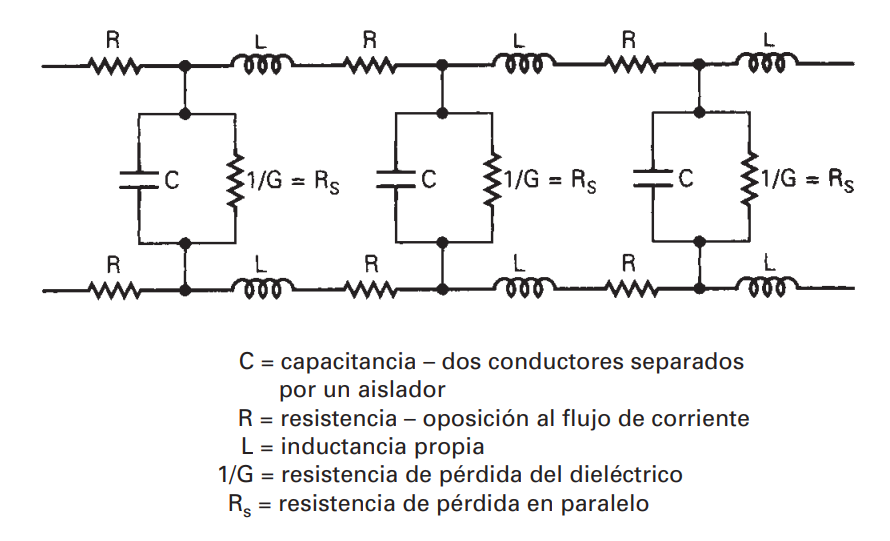
\includegraphics[width=0.8\textwidth]{imagenes/circ_lt.png}
                \caption{Línea de transmisión de dos hilos paralelos; circuito eléctrico equivalente y modela las perdidas}
                \label{fig:circ_lt}
            \end{figure}

            \paragraph{Características de transmisión:}

            Las características de transmisión de una línea se llaman constantes secundarias, y se calculan a partir de las cuatro constantes primarias. Las constantes secundarias son la impedancia característica y la constante de propagación.

            \begin{itemize}
                \item \textbf{Impedancia característica}

                Para que haya una transferencia máxima de energía de la fuente a la carga, es decir, que no haya energía reflejada, una línea de transmisión debe terminar en una carga puramente resistiva, igual a la impedancia característica de ella. La impedancia característica, $Z_o$, de una línea de transmisión es una cantidad compleja que se expresa en ohms, y que en el caso ideal es independiente de la longitud de la línea y que no se puede medir. 
                
                Esa impedancia característica, se define como la impedancia vista hacia una línea de longitud infinita, o la impedancia vista hacia una línea de longitud finita que termina en una carga puramente resistiva igual a la impedancia característica de la línea. Una línea de transmisión almacena energía en su inductancia y capacitancia distribuidas. Si la línea es infinitamente larga, puede almacenar energía en forma indefinida; la energía procede de la fuente, entra a la línea y nada regresa. Por lo mismo, la línea funciona como un resistor que disipa toda la energía. Se puede simular una línea infinita si una línea finita termina en una carga puramente resistiva igual a $Z_o$; toda la energía que entra de la fuente a la línea se disipa en la carga (esto supone que la línea es totalmente sin pérdidas).

                \item \textbf{Constante de propagación}

                La constante de propagación, que a veces se le llama coeficiente de propagación se usa para expresar \textbf{ la atenuación (pérdida de señal)} y el desplazamiento de fase por unidad de longitud de una línea de transmisión. Cuando una onda se propaga por una línea de transmisión disminuye su amplitud con la distancia recorrida.\textbf{ Se usa la constante de propagación para determinar la reducción de voltaje o de corriente con la distancia, cuando una onda EMT se propaga por una línea de transmisión}. Cuando la línea es de longitud infinita, toda la potencia incidente se disipa en la resistencia del conductor al avanzar la onda por la línea. Por consiguiente, con una línea de longitud infinita, o una que se vea infinitamente larga, como puede ser una línea finita terminada en una carga equilibrada ($Z_o = Z_L$), no regresa o se refleja energía alguna hacia la fuente. 

                La ecuación de la constante de propagación es:

                \begin{gather}
                    \gamma = \alpha + j \beta \label{eq:cons_propagacion}
                \end{gather}

                Siendo, 
                \begin{align*}
                    \gamma &= \text{constante de propagación} \\
                    \alpha &= \text{ coeficiente de atenuación (nepers por unidad de longitud)} \\
                    \beta &= \text{coeficiente de desplazamiento de fase (radianes por unidad de longitud)}
                \end{align*}
                
                La constante de propagación es una cantidad compleja y se define como sigue 

                \begin{gather}
                    \gamma = \sqrt{(R+j\omega L)(G+j \omega C)} \label{eq:cons_propagacion_2}
                \end{gather}

                Como en cada distancia igual a la longitud de onda se produce un desplazamiento de fase de $2 \pi$,

                \begin{gather}
                    \beta = \dfrac{2 \pi}{\lambda} \label{eq:coef_desplazamiento}
                \end{gather}

                A frecuencias intermedias y de radio, $\omega L > R$ y $\omega C > G$, entonces

                \begin{gather}
                    \alpha= \dfrac{R}{2Z_o}+\dfrac{GZ_o}{2} \label{eq:coef_atenuacion} \\[0.2cm]
                    \beta = \omega \sqrt{LC}
                \end{gather}

                La distribución de corriente y voltaje a lo largo de una línea de transmisión que termina en una carga igual a su impedancia característica (una línea equilibrada) se calculan con las siguientes fórmulas

                \begin{gather}
                    I=I_s e^{-l\gamma} \label{eq:corriente} \\[0.2cm]
                    V=V_s e^{-l\gamma} \label{eq:voltaje}
                \end{gather}

                En las que, 

                \begin{align*}
                    I_s&= \text{corriente en el extremo de la línea que da la fuente (amp)} \\[0.2cm]
                    V_s&= \text{voltaje en el extremo de la línea que da la fuente (volts)} \\[0.2cm]
                    \gamma&= \text{constante de propagación} \\[0.2cm]
                    I&= \text{distancia de la fuente hasta donde se determina la corriente o el voltaje} \\[0.2cm]
                \end{align*}

                Para una carga equilibrada $Z_L=Z_o$ y para determinada longitud de cable $l$, la pérdida de voltaje o corriente de señal es la parte real de $\gamma l$, y el desplazamiento de fase es la parte imaginaria. 

                
            \end{itemize}

        \subsubsection{Propagación de ondas en línea de transmisión}

            Las ondas electromagnéticas viajan a la velocidad de la luz cuando se propagan en el vacío, y casi a la velocidad de la luz cuando lo hacen a través del aire. Sin embargo, en las líneas metálicas de transmisión, donde el conductor suele ser cobre, y en los materiales dieléctricos, la velocidad varía mucho de acuerdo con el tipo de cable, y una onda electromagnética viaja con mucha mayor lentitud.

            \paragraph{Factor de velocidad}

                El factor de velocidad (llamado a veces constante de velocidad) se define como la relación de la velocidad real de propagación a través de determinado medio, entre la velocidad de propagación a través del espacio vacío. La definición matemática del factor de velocidad es:

                \begin{gather}
                    V_f=\dfrac{V_p}{c} \label{eq:factor_velocidad}  
                \end{gather}

                donde,

                \begin{align*}
                    V_f&= \text{factor de velocidad (adimensional)} \\[0.2cm]
                    V_p&= \text{Velocidad real de propagación (metros por segundo)} \\[0.2cm]
                    c&= \text{Velocidad de propagación a través del espacio vacío} (c=3x10^8 m/s)
                \end{align*}

                y $V_f x c = V_p$

                La velocidad a la que viaja una onda electromagnética por una línea de transmisión depende de la constante dieléctrica del material aislante que separa a los dos conductores. El factor de velocidad se calcula en forma muy aproximada con la fórmula:

                \begin{gather}
                    V_f= \dfrac{1}{\sqrt{\epsilon_r}}
                \end{gather}
            
                en la que $\epsilon_r$ es la constante dieléctrica del material dado (la permitividad del material en relación con la permitividad en el vacío; es la misma relación $\dfrac{\epsilon}{\epsilon_o}$). 
                
                La constante dieléctrica es tan sólo la permitividad relativa de un material.

                La constante dieléctrica depende del material que se use. Los inductores almacenan energía magnética, y los capacitores almacenan energía eléctrica. Se necesita un tiempo finito para que un inductor o un capacitor tome o ceda energía. Por consiguiente, la velocidad con la que se propaga una onda electromagnética por una línea de transmisión varía de acuerdo con la inductancia y la capacitancia. Se puede demostrar que ese tiempo de carga es $T = \sqrt{LC}$ . Así, la inductancia, capacitancia y velocidad de propagación se relacionan mediante la fórmula

                $$ Velocidad \times tiempo = distancia$$

                Por consiguiente, 

                \begin{gather}
                    V_p = \dfrac{distancia}{tiempo} = \dfrac{D}{T} \nonumber \\[0.2cm] 
                    \text{ Al Sustituir el tiempo se obtiene } \, V_p = \dfrac{D}{\sqrt{LC}} \nonumber\\[0.2cm] 
                    \text{Si la distancia se normaliza a 1 m, la velocidad de propagación de una línea sin pérdidas es} \nonumber\\[0.2cm] 
                    V_p = \dfrac{1 \, m}{ \sqrt{LC}} = \dfrac{1}{\sqrt{LC}} m/s \label{eq:velocidad_real_propagacion} \\[0.2cm]
                    \text{ donde $V_p =$ velocidad de propagación (metros por segundo} \nonumber\\[0.2cm]
                    \sqrt{LC} = \text{segundos} \nonumber
                \end{gather}


            \paragraph{Líneas de retardo}

                Las líneas de retardo son líneas de transmisión diseñadas en forma intencional para introducir un retardo de tiempo en la trayectoria de una onda electromagnética. La cantidad de retardo es función de la inductancia y la capacitancia de la línea de transmisión. La inductancia se opone a cambios de corriente, al igual que los tiempos de carga y descarga de la capacitancia. El retardo se calcula como sigue:

                \begin{gather}
                    t_d= LC \, (segundos) \label{eq:ti_retardo}
                \end{gather}

                \begin{align*}
                    \text{donde } \, t_d &= \text{retardo (segundos} \\[0.2cm]
                    L &= \text{inductancia (henrys} \\[0.2cm]
                    C &= \text{capacitancia (farads} 
                \end{align*}

                Si la inductancia y la capacitancia se expresan por unidad de longitud de línea de transmisión, por ejemplo por metro o por pie, el retardo también será por unidad de longitud; por ejemplo, 1.5 ns/metro. 
                La demora introducida por un tramo de cable coaxial se calcula con la siguiente fórmula:

                \begin{gather}
                    t_d=1.016 \, \epsilon \label{eq:ti_retardo_2}
                \end{gather}

                en la que $\epsilon$ es la constante dieléctrica del cable.

        \subsubsection{Pérdidas en líneas de transmisión}

            Para fines de análisis, las líneas de transmisión se consideran, con frecuencia, sin pérdidas. Sin embargo, en realidad hay varias formas en las que se pierde la energía en una línea de transmisión. Están las pérdidas en el conductor, pérdidas por radiación, pérdidas por calentamiento del dieléctrico, pérdidas por acoplamiento y efecto de corona.

            \paragraph{Pérdidas en el conductor}

                Como la corriente pasa por una línea de transmisión, y ésta tiene una resistencia finita, hay una pérdida inherente e inevitable de potencia. A veces a esto se le llama pérdida en el conductor o pérdida por calentamiento del conductor, y es tan sólo una pérdida de la forma $I^2R$. Como la resistencia está distribuida en una línea de transmisión, la pérdida en el conductor es directamente proporcional a la longitud de la línea. También, ya que la disipación de potencia es directamente proporcional al cuadrado de la corriente, la pérdida en el conductor es inversamente proporcional a la impedancia característica. Para reducir las pérdidas en el conductor no hay más que acortar la línea de transmisión o usar un alambre de mayor diámetro (téngase en cuenta que al cambiar el diámetro del alambre también cambia la impedancia característica y, en consecuencia, la corriente).

                La pérdida en el conductor depende algo de la frecuencia, debido a una acción llamada efecto de superficie. Cuando pasa la corriente por un alambre redondo aislado, el flujo magnético asociado con ella tiene la forma de círculos concéntricos. Esto se ve en la fig. \ref{fig:perdidas_conductor}. Se puede demostrar que la densidad de flujo cerca del centro del conductor es mayor que cerca de la superficie. Entonces, las líneas de flujo cercanas al centro del conductor encierran la corriente y reducen la movilidad de los electrones encerrados. Es una forma de autoinductancia, y hace que la inductancia cercana al centro del conductor sea mayor que en la superficie. Así, en las radiofrecuencias, la mayor parte de la corriente pasa por la superficie y no cerca del centro del conductor. Esto equivale a reducir el área transversal del conductor, y a aumentar la oposición al flujo de corriente (es decir, a aumentar la resistencia). La oposición adicional tiene ángulo de fase igual a $0^\circ$, y en consecuencia es una resistencia, y no una reactancia. Así, la resistencia en ca del conductor es proporcional a la raíz cuadrada de la frecuencia. La relación de la resistencia en ca entre la resistencia en cd de un conductor se llama relación de resistencias. Arriba de más o menos 100 MHz, se puede eliminar por completo el centro de un conductor, sin tener absolutamente efecto alguno sobre la pérdida en el conductor o la propagación de la onda electromagnética.

                \begin{figure}[H]
                    \centering
                    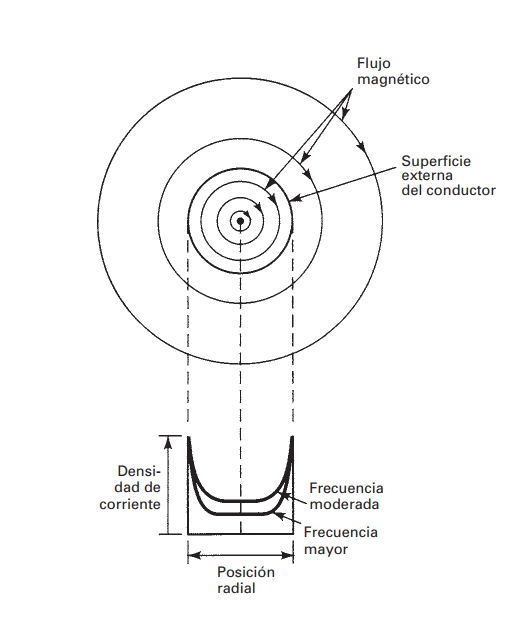
\includegraphics[width=0.5\linewidth]{imagenes/perdidas_conductor.png}
                    \caption{Conductor redondo aislado mostrando las líneas de flujo magnético, distribución de corrientes y el efecto de superficie}
                    \label{fig:perdidas_conductor}
                \end{figure}

                Las pérdidas en el conductor, en las líneas de transmisión, varía desde una fracción de decibel por 100 m en los cables coaxiales rígidos con dieléctrico de aire, hasta 200 dB por 100 m en una línea flexible de dieléctrico rígido. Tanto las pérdidas $I^2R$ como las del dieléctrico son proporcionales a la longitud, con frecuencia se agrupan y se expresan en decibeles de pérdida por unidad de longitud, es decir, dB/m.

            \paragraph{Pérdida por calentamiento del dieléctrico}

                Una diferencia de potencial entre los dos conductores de una línea de transmisión causa el calentamiento del dieléctrico. El calor es una forma de energía que se debe tener en cuenta cuando se propaga energía por la línea. Para las líneas con dieléctrico de aire, la pérdida por calentamiento es despreciable. Sin embargo, con las líneas rígidas el calentamiento del dieléctrico aumenta con la frecuencia.

            \paragraph{Pérdida por radiación}

                Si la separación entre los conductores de una línea de transmisión es una fracción apreciable de una longitud de onda, los campos electrostático y electromagnético que rodean al conductor hacen que la línea funcione como si fuera una antena, y transfiera energía a cualquier material conductor cercano. La cantidad de energía irradiada depende del material dieléctrico, la distancia entre conductores y la longitud de la línea. Las pérdidas por radiación se reducen blindando el cable en forma adecuada. Así, los cables coaxiales tienen menores pérdidas por radiación que las líneas de dos alambres paralelos. La pérdida por radiación también es proporcional a la frecuencia.

            \paragraph{Pérdida por acoplamiento}

                La pérdida por acoplamiento se presenta siempre que se hace una conexión con o de una línea de transmisión, o cuando se conectan dos tramos separados de línea de transmisión. Las conexiones mecánicas son discontinuidades, es decir, lugares donde se unen materiales distintos. Las discontinuidades se tienden a calentar, irradian energía y disipan potencia.

            \paragraph{Efecto corona (o efecto de arco voltaico)}

                El arco voltaico es una descarga luminosa que se produce entre dos conductores de una línea del dieléctrico aislante. En general, una vez que se produce el efecto de arco voltaico o efecto corona, la línea de transmisión se destruye.


        \subsubsection{Resistividad}

            La resistividad es la resistencia eléctrica específica de un determinado material. Se designa por la letra griega rho minúscula ($\rho$) y se mide en ohmios $\cdot$ metro ($\Omega \cdot m$).

            Su valor describe el comportamiento de un material frente al paso de corriente eléctrica: un valor alto de resistividad indica que el material es un aislante mientras que un valor bajo indica que es un conductor.

            \begin{figure}[H]
                \centering
                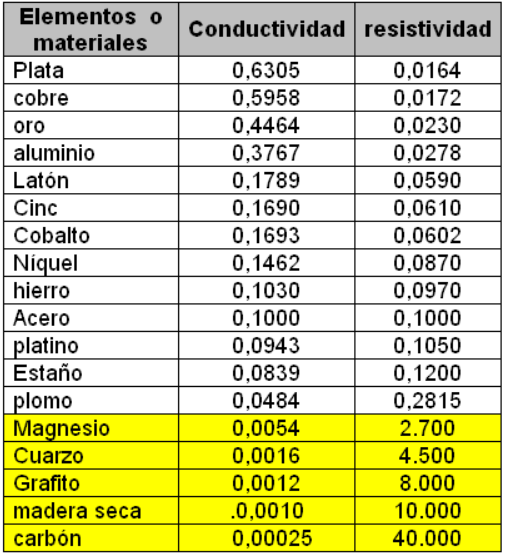
\includegraphics[width=0.5\linewidth]{imagenes/resistividad.png}
                \caption{Tabla de resistividad de algunos elementos}
                \label{fig:resistividad}
            \end{figure}










                
\newpage